%%%%%%%%%%%%%%%%%%%%%%%%%%%%%%%%%%%%%%%%%%%%%%%%%%%%%%%%%%%%%%%%%%%%%%%
%                                                                     %   
%    Latex Template Literature Review                                 %
%    Z. Wang 
%    Oct 2024
%    University of Exeter                                             %
%                                                                     %
%%%%%%%%%%%%%%%%%%%%%%%%%%%%%%%%%%%%%%%%%%%%%%%%%%%%%%%%%%%%%%%%%%%%%%%
\documentclass[11pt,a4paper]{article}

\usepackage{amsmath}
\usepackage{amsfonts}
\usepackage{geometry}
\usepackage{graphicx}
\usepackage{fancyhdr}
\usepackage{setspace}
\usepackage{amssymb}
\usepackage{booktabs}
\usepackage{enumitem}
\usepackage{multirow}

\usepackage{graphicx}
\usepackage{float}
\usepackage[section]{placeins}
% disable author name being replaced with underscores in bibtex
% \usepackage[style=ieee,dashed=false]{biblatex}
% unticked checkbox
\newlist{checkbox}{itemize}{2}
\setlist[checkbox]{label=$\square$}
% ticked checkbox
\newlist{checkbox_t}{itemize}{2}
\setlist[checkbox_t]{label=$\text{\rlap{$\checkmark$}}\square$}


% Page layout settings
\geometry{
    a4paper,
    left=20mm,
    right=20mm,
    top=25mm,
    bottom=25mm
}

%%%%%%%%%%%%%%%%%%%%%%%%%%%%%%%%%%%%%%%%%%%%%%%%%%%%%%%%%%%%%%%%%%%%%%
%%%%%%%%%%%%%%%%%%%%%%%%%%%%%%%%%%%%%%%%%%%%%%%%%%%%%%%%%%%%%%%%%%%%%%
\begin{document}
\singlespacing  % Set the document to single line spacing
\thispagestyle{empty} % remove page number for the cover page

\begin{center}
{\bf \LARGE An Explainable AI Model for IoMT Network Attack Detection}\\[0.5cm]
    \textbf{Ralph Lickley} \\[0.2cm]
    \textbf{Student ID:} 730030331 \\[1cm]
    \textbf{Email:} rl665@exeter.ac.uk \\[1cm]
\end{center}

\section*{Abstract}
\noindent 
The Internet of Medical Things (IoMT) has become increasingly more integrated into healthcare delivery in recent years. Along with it’s many benefits in improving healthcare efficiency, it has also opened the medical industry to a wide variety of new cyberattacks, raising many concerns involving the privacy of patients data as well as their safety when receiving medical treatment. A common solution to this has been Machine Learning (ML) based Intrusion Detection Systems (IDS), which have provided high accuracy in classifying malicious network traffic in many IoT applications, and some IoMT scenarios. However, more complex ML based IDS are fundamentally less interpretable, this is an issue as it prevents trust from both patients and medical professionals. This project will address this critical gap through the design, implementation, and evaluation of a deep learning model incorporating Explainable Artificial Intelligence (XAI) that detects network attacks specific to an IoMT network.
\vspace*{\fill}

% \begin{checkbox}
%     % \item {\bf I have not used any GenAI tools in preparing this assessment.}
%     \item {\bf I certify that all material in this dissertation which is not my own has been identified.}
% \end{checkbox}

%  Uncomment to tick the decalaration
% \begin{checkbox_t}
%     \item {\bf I have not used any GenAI tools in preparing this assessment.}
%     \item {\bf I certify that all material in this dissertation which is not my own has been identified.}
% \end{checkbox_t}

\vspace{1em}
% {\bf\noindent Signature:} \hrulefill

\newpage
% reset page number
\clearpage
\pagenumbering{arabic} 
%%%%%%%%%%%%%%%%%%%%%%%%%%%%%%%%%%%%%%%%%%%%%%%%%%%%%%%%%%%%%%%%%%%%%%
%
%    Section 1
%
%%%%%%%%%%%%%%%%%%%%%%%%%%%%%%%%%%%%%%%%%%%%%%%%%%%%%%%%%%%%%%%%%%%%%%
\section{Introduction}

Smart and connected medical devices are increasingly integrated into the delivery of healthcare services, leading to the development of the Internet of Medical Things (IoMT), a subset of the Internet of Things (IoT) encompassing medical equipment and devices such as heart rate and cardiovascular monitoring, remote medicine alert systems, and temperature tracking. 
IoMT technology offers many advantages by enabling continuous monitoring of patients’ health. This assists healthcare professionals in making remote diagnoses and better informing their clinical decisions; for example, data collected from IoMT devices has been used to predict patients’ risk of heart disease \cite{baseer2024healthcare}. With the growing digitalisation of healthcare systems, there has been a significant increase in cyberattacks targeting medical infrastructure. 
According to the HIPAA Journals’ report, there have been 546 healthcare breaches that affect more than 500 people so far in 2025 \cite{hipaajournal}. This, coupled with the sensitive nature of medical data, raises major concerns about patients’ privacy, where patients’ personal data may be exposed, as well as potential concerns about patients’ safety, given that IoMT devices are used to deliver treatments. 
Recent research has shown that Machine Learning (ML) can be effectively used to detect network attacks by analysing network traffic \cite{althubitiids, agarapneuralids, PRAMILARANI2024111125}. 
Compared to traditional network attack detection methods, such as signature-based systems, ML techniques offer significant improvements in detecting unknown attack types, this is because they are able to recognise complex patterns in network traffic attributed to malicious activity \cite{fidelisecurity}.
However, one problem faced by complex ML techniques is their lack of interpretability in decision-making; in the context of healthcare systems, this interpretability is crucial, as medical staff and patients need to trust that IoMT networks are secure. 
To address the lack of interpretable ML models, this project will develop a Deep Learning IDS and use Explainable Artificial Intelligence (XAI) techniques to make its decisions more interpretable in IoMT systems. This ensures that users of the system can understand and trust the model while still achieving high detection accuracy. The proposed model will be trained and evaluated using the CIC2024 IoMT dataset, a publicly available dataset synthesised by the Canadian Institute for Cybersecurity \cite{dadkhah2024ciciomt2024}. This dataset has been specifically designed to develop and benchmark network attack detection models in IoMT environments, incorporating a various IoMT devices and a wide variety of both benign and malicious network traffic.

\section{Literature Review}

\subsection{IoMT Architecture and Security Concerns}
IoT, and subsequently IoMT systems, are typically divided into three primary layers: perception, network, and applications \cite{almulla2025layered}.

In the perception (physical) layer, we have the actual medical sensors and wearable devices that collect information from patients, such as tracking cardiovascular and heart health, temperature, and sleep patterns. This layer faces potential vulnerabilities, with the potential for tampering and false data collection, which could ultimately lead to incorrect diagnoses based on incorrect data. 

The network layer enables these devices to communicate with other devices in the IoMT network using protocols such as Wi-Fi and Bluetooth. This layer is susceptible to attacks such as DoS and DDoS, which can lead to disruptions in treatment and pose an immediate risk to patients' safety when IoMT devices are unable to operate. Man-in-the-middle attacks at this layer can also lead to data breaches, compromising the confidentiality of sensitive patient and medical staff data. The IDS discussed later in this literature review, as well as the IDS that will be developed in this project are primarily based on this network layer

Moving to the application layer, we find software vulnerabilities where cyber threats, such as phishing and ransomware, can lead to interruptions in medical care and further data breaches. 

\begin{figure}[H]
    \centering
    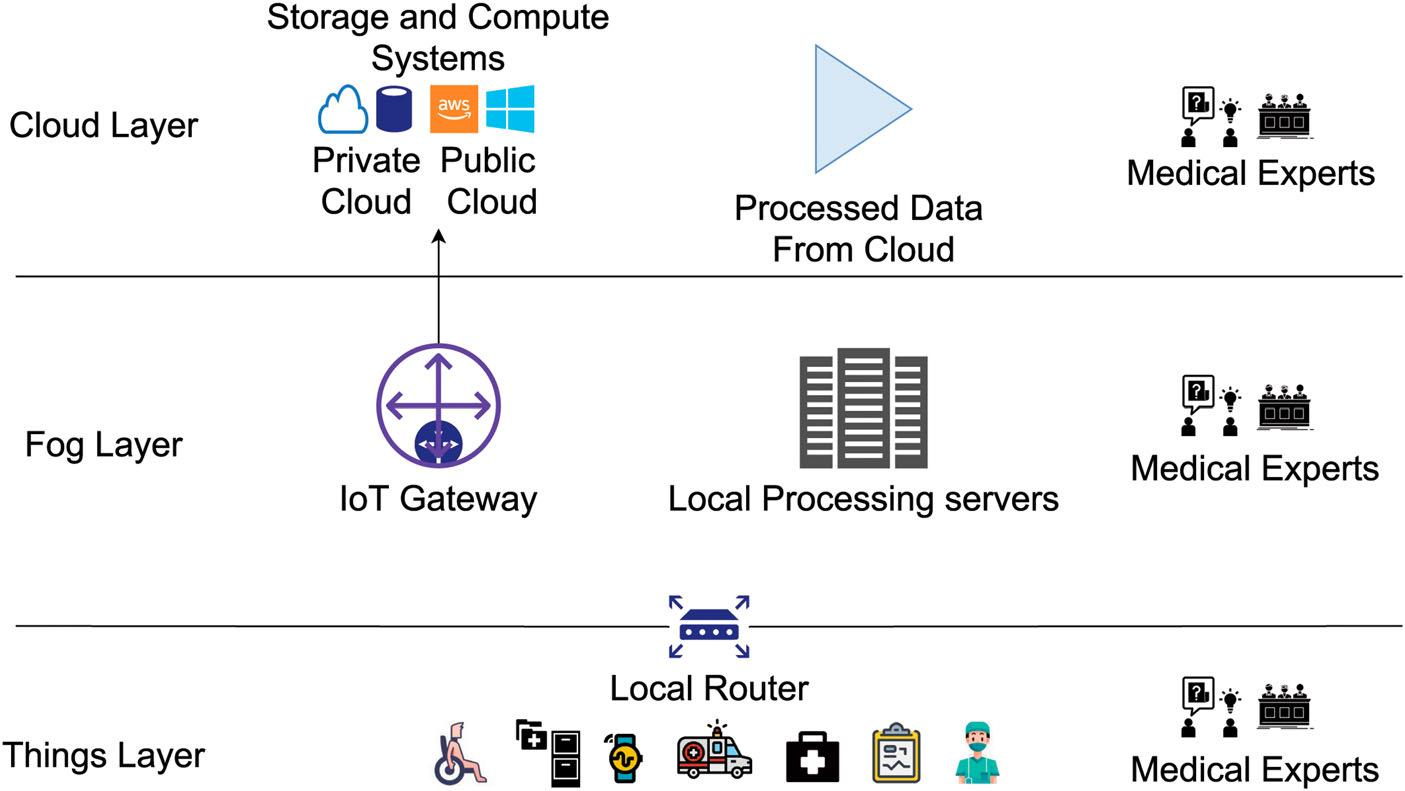
\includegraphics[width=0.6\linewidth]{images/iomt-architecture.jpg}
    \caption{Illustration of layers in an IoMT system. Source: \cite{purelogics}}
    \label{fig:IoMTLayers}
\end{figure}

Across these layers, there are three clear points of risk for IoMT technology: patients' data privacy, patients' safety, and disruption to medical systems. 

The variety of areas that are vulnerable in these systems highlights the need for a more rigorous and trustworthy cybersecurity system to reduce the number of successful attacks. Effective Intrusion Detection System (IDS) is an essential tool for preventing the wide variety of attacks that can IoMT networks face.


\subsection{ML-Driven IDS}
Traditional Intrusion Detection Systems (IDS) such as signature based methods are not well-suited to the field of IoT networks due to various unknown attack types, this has lead to research in recent years primarily being focused on hybrid Machine Learning (ML) methods for detecting network attacks, including Random Forest and SVM \cite{da2019internet}. 
These ML-based systems aim to analyse large amounts of network traffic and distinguish between benign and malicious activity. 
This section will focus on reviewing the most well-documented models used and how their performance is evaluated in various IDS. Continuing with the shift toward ML-driven IDS approaches, early ML based IDS explored the efficacy of algorithms such as Decision Trees and SVMs, both of which achieve promising results when tested on benchmark datasets. For example one IDS uses a Hybrid Decision Tree tested and evaluated on the NSL-KDD dataset \cite{5356528} achieves 83\% accuracy and 0.83 F1 score, outperforming other ML methods such as SVM and KNN \cite{taghavinejad2020intrusion}. However, this model does not distinguish between attack types such as DoS, MITM, and others, which is desirable for IoMT security; the authors suggest future work to address this limitation. 
Deep learning methods provide a solution to this, a deep reinforcement learning model was developed and tested alongside traditional ML methods to detect malicious network traffic in IoT networks. Using the NSL-KDD dataset \cite{5356528}, the best performing model was the Double Deep Q-Network (DDQN) achieving an accuracy of around 80\% and F1 score of 0.91\cite{lopez2020application}. Comparing this with the Hybrid Decision Tree, it is clear that this form of deep reinforcement learning excels in attack detection. A noticeable drawback of deep learning here is the time taken to train the model compared to traditional ML as well as the lack of interpretability it provides. 
In \cite{kulshresthap}, an ML IDS which is specific to IoMT is presented. Using the ToN\_IoT Network dataset, the authors carried out comparisons between eleven different attack classification model. The most effective classifier was found to be Adaptive Boosting ensemble technique, achieving an accuracy of 99.18\%. However, one potential gap in the implementation of this model is the dataset used, it has not been specifically created to reflect IoMT networks, rather more general IoT networks. This could cause the model to face challenges in a real world IoMT environment, where IoMT devices make use of specific lightweight protocols such as Bluetooth and MQTT.

\subsection{Explainable Artificial Intelligence (XAI) in IDS}
Explainable Artificial Intelligence (XAI) refers to a set of tools which aim to make the predictions made by a deep learning model understandable to humans, this is in the form of showing the features the model decides played the biggest role in making the final prediction. Obviously, in a healthcare setting, the ability to trust is essential with the IDS system securing an IoMT network because we do not want to risk genuine medical communications being interrupted, which could lead to disruptions to patients treatment. However, we still want to accurately prevent malicious attacks that could cause reduced patient safety and sensitive medical data being compromised. Therefore, integrating XAI into a deep learning IDS allows the healthcare industry to understand and validate a the predictions of the model.
The two main types of XAI models are model-specific and model-agnostic. Model specific XAI is suited to a specific group of models, meaning they offer a deep insight into the models decision making, however they cannot be applied to a wide variety of model types. Model agnostic techniques are the opposite, they can be applied to many model types with a less in-depth insight. \cite{devireddy2025comparative}.
Some examples of XAI techniques are LIME and SHAP. LIME (Local Interpretable Mode-agnostic Explanations) is an algorithm proposed in 2016, it explains the prediction of a classifier (model-agnostic) though approximating it with a simpler and interpretable model \cite{ribeiro2016should}. Later, SHAP (Shapley Additive exPlanations) was introduced in 2017 \cite{lundberg2017unified}, similar to LIME, it is a model-agnostic algorithm that determines how each feature contributes to a models output.
Recent studies and research demonstrate that XAI models, such as LIME and SHAP are effective in explaining predictions made by IDS systems. 
In \cite{wang2020explainable}, researchers successfully introduce an explainable machine learning framework for IDS, this framework was built around the SHAP method and used the NSL-KDD dataset \cite{5356528} to evaluate the models performance. However, this paper mentions the frameworks limitations and highlights the need for more datasets to be tested to improve the explainability. 
A deep learning based IDS is proposed in \cite{SHARMA2024121751}, the authors integrate XAI models including both LIME and SHAP. This paper evaluates the performance on both the NSL-KDD dataset as well as UNSW-NB15, demonstrating that XAI models make these deep learning models more transparent and trustworthy.
There is limited work in applying XAI techniques specifically to IoMT scenarios, addressing this gap will allow the development of more trustworthy IDS models in healthcare settings that use IoMT networks.

\subsection{Evaluation Datasets and Benchmarks}
The accuracy and reliability of Machine Learning (ML) based Intrusion Detection Systems (IDS) are primarily dependent on the quality and the realism of the data used to train, validate and test the model. This is especially important in IoMT settings because the data transmitted in these networks are fundamentally more sensitive than a typical IoT network, making the need for secure communications essential. This section will critically evaluate the available datasets that have previously been used in ML-driven IDS models, discuss the limitations and justify the selection of the CIC2024 IoMT Dataset for this projects specific focus.
The dataset, NSL-KDD \cite{5356528}, frequently mentioned in the previous sections of this literature review, has been used extensively in training IDS models. This dataset was synthesised to improve upon its predecessor and has been able to produce promising results in many research application. However, this dataset has drawbacks such as its high redundancy of its records, which can lead to poor generalization in ML models \cite{revathi2013detailed}. This dataset would not be suitable for the model proposed in this report because it does not reflect an accurate IoMT system.
Newer datasets provide significant improvements of NSL-KDD, one notable example is the CICIDS2017 dataset, this dataset includes more realistic network traffic in IoT networks. However, this would also not be suited to IoMT systems due to it not containing common examples of network traffic such as lightweight protocols MQTT and Bluetooth which are used by IoMT devices. 
To maximise the realism of the data used to train the proposed model, this project will use the CIC2024 IoMT Dataset \cite{dadkhah2024ciciomt2024}. This dataset was specifically synthesised for benchmarking security systems for IoMT. It involves traffic types missing from the previously mentioned datasets including common protocols used by IoMT such as MQTT and Bluetooth. This dataset also provides a wide variety of current and relevant attack vectors faced by real world IoMT networks.
\begin{figure}[H]
    \centering
    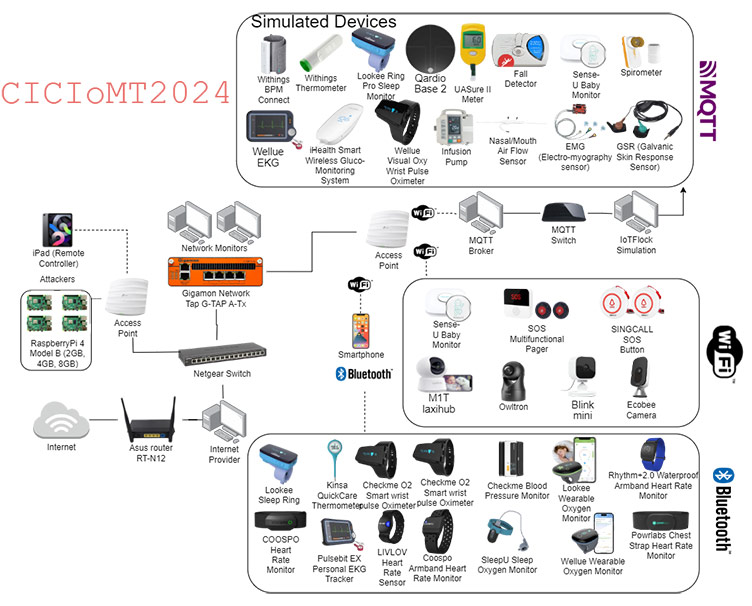
\includegraphics[width=0.6\linewidth]{images/inline-topology.jpg}
    \caption{CICIoMT2024 topology. Source: \cite{dadkhah2024ciciomt2024}}
    \label{fig:CIC2024IoMT_Toplogy}
\end{figure}
The structure of the dataset will guide the development of this model. Due to the large class imbalance where a large portion of the network traffic is of type DDoS, the evaluation of the model will need to incorporate various metrics such as F1-score, Recall, and Precision to ensure the model minimises false classifications.

\section{Project Specification}
\subsection{Motivation}
The use of IoMT systems continues to spread in the field of modern healthcare, with many routine health checks now able to be performed remotely and continuously. Unfortunately, with this increase of its use, there has also been an increase in the amount of cyber-attacks focused on healthcare services \cite{hipaajournal}. The main motivation of this project is to address the lack of trust that can be placed in Machine Learning based Intrusion Detection Systems, through developing an explainable model who’s decisions can be verified and understood.


\subsection{Aims and Objectives}
The overarching goal of this project is to design, implement and evaluate an XAI IDS model that produces accurate and reliable attack detection, specifically in a realistic IoMT environment.  
\\
The primary objectives of this project are: 
\begin{itemize}
    \item Obtain and prepare the CIC2024 IoMT Dataset, ensuring it is ready for model training, including necessary preprocessing steps to address features of the dataset such as the class imbalance.
    \item Design and implement the chosen Deep Learning IDS model, then train it using the now prepared dataset. Achieving satisfying evaluation metrics such as F1 score, before integrating the explainable AI into the model.
    \item Integrate XAI techniques into the model (LIME and SHAP), then conduct analysis on the output of both methods to determine if they methods consistently flag the same features as the most crucial for predicting a given attack type. The robustness of the explainable elements can also be validated against the known characteristics of certain attacks. 
\end{itemize}

\subsection{Gantt Chart Timeline}
\begin{figure}[H]
    \centering
    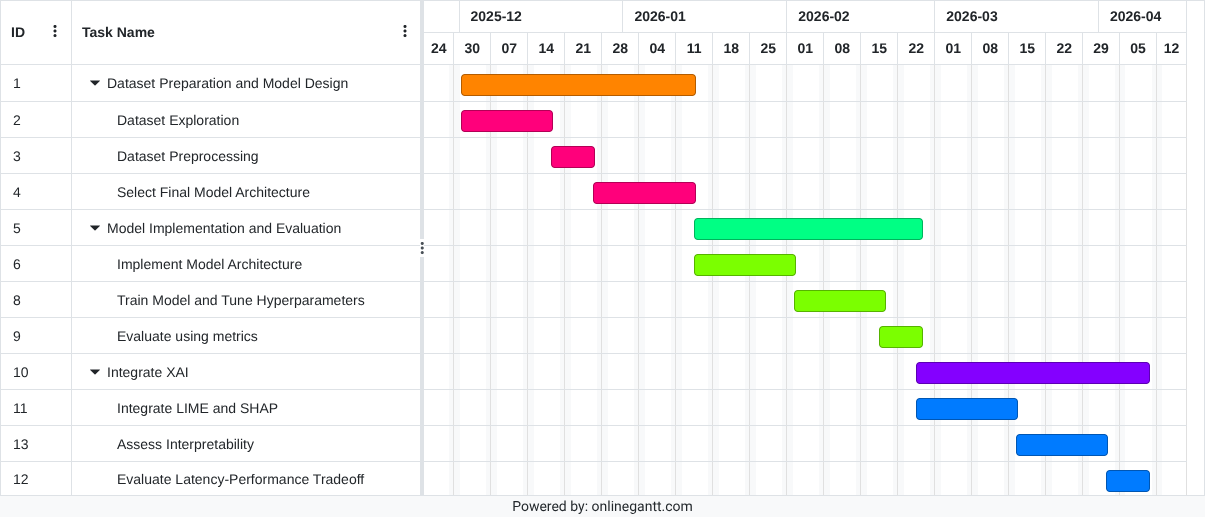
\includegraphics[width=1.0\linewidth]{images/ganttchart2.png}
    \caption{Gantt Chart of the projects timeline}
\end{figure}

\subsection{Methodology and Implementation Plan}
\subsubsection{Dataset}
\begin{itemize}
    \item The project will make use of the CIC2024 IoMT dataset, this is due to its focus on IoMT networks as well as its up-to-date nature, and the variety of IoMT relevant attack types it simulates.
    \item Dataset cleaning will involve the removal of any redundant features in the dataset, and create some categorical encodings for malicious and benign traffic.
    \item Address class imbalance, possibly using SMOTE to balance dataset, as the majority class by far in the dataset is DDoS and DoS attacks.
    \item Split the dataset into subsets: training, validation, and testing. Ready for the models training and evaluation process.
\end{itemize}

\subsubsection{Model Design}
A Deep Neural Network is chosen as the model to be implemented for this IDS, this is because it was among the strongest performers when tested on the chosen dataset \cite{dadkhah2024ciciomt2024}, achieving solid F1 scores in 2, 6 and 19 class classifications, narrowly being beaten by the RandomForest model. The validation set, reserved in the dataset preprocessing will be used for hyperparameter tuning, to maximise performance.

\subsubsection{XAI Integration}
To compare the  both SHAP and LIME will be tested on the model. Both will be used to show which features were the most important when making a prediction.

\subsection{Evaluation and Success Criteria}
IDS Model performance will be measured using F1-score, aiming to achieve a score greater than 0.85 is a reasonable target, this would indicate that the model strikes a strong balance between both precision and recall when detecting malicious network traffic.
The benchmark for the proposed model will be based on existing results published on the paper for the CIC2024 IoMT Dataset, primarily the DNN mentioned and Random Forest model.
To measure the success of the integration of XAI techniques (LIME and SHAP), there will be a comparison between the explanations provided by both methods to see if they both identify the same features across attacks. 


\subsection{Risks and Ethical Considerations}
The dataset that has been selected for this project does have a large class imbalance, with there being substantially more entries of DDoS and DoS network traffic compared to other attack types and benign traffic. This could lead to the model incorrectly classifying malicious network traffic as DDoS and DoS attacks resulting in inaccurate attack detection, putting patient safety at risk if medical systems are interrupted. To combat this, the model could employ preprocessing techniques such as SMOTE (Synthetic Minority Over-sampling Technique) during training.
Sourcing of the data needed to train this model is also an ethical concern, due to the data transferred on IoMT networks potentially being sensitive and private to patients. The project’s use of the CIC2024 IoMT Dataset is an intentional answer to this concern, since it is a publicly available dataset that has been synthesised, there is no handling or storage of real patients’ data.
\newpage
\bibliographystyle{IEEEtran}
\bibliography{main.bib}
\end{document}

